\documentclass{article} % For LaTeX2e
\usepackage{cos424,times}
\usepackage{url}
\usepackage{graphicx}
\usepackage{hyperref}
\usepackage{amsmath, bbold}
\usepackage{bm}
\usepackage{biblatex}
\bibliography{bib.bib}

\newcommand{\e}{\text{e}}
\newcommand{\bt}{\mathbf}

\title{Kaggle Competition: Flavors of Physics}


\author{
Kenan Farmer\\
Computer Science\\
\texttt{kfarmer@} \\
\And
Charles Stahl \\
Physics \\
\texttt{cnstahl@} \\
\And
Meir Hirsch\\
Computer Science \\
\texttt{ehirsch@} \\
}

\newcommand{\fix}{\marginpar{FIX}}
\newcommand{\new}{\marginpar{NEW}}

\begin{document}

\maketitle

\subsection*{Introduction}

The Large Hadron Collider (LHC) is a particle accelerator in Europe. It is designed to test high energy physics, specifically the standard model. The standard model is our current understanding of how the universe behaves. 

One prediction of the standard model is conservation of lepton number \cite{griff87}. Lepton number is the total number of leptons minus the total number of antileptons,
\begin{align}
L=n_{\ell }-n_{\overline {\ell }}~.
\end{align}
There are two types of leptons: charged leptons such as electrons muons and tauons, and neutral leptons, which are called neutrinos. They can be further divided into families. Electrons and electron neutrinos are in the electron family, etc.

Neutrinos have a very small mass, six to nine orders of magnitude smaller than the electron mass. If their mass were exactly zero, Lepton number would be conserved for each family individually. However, the minuscule neutrino mass allows some lepton family number violations. 

The $\tau\to\mu\mu\mu$ reaction is one such violation. 

\subsection*{Data Description}

This will be a classification problem using all real data.

\subsection*{Methodologies to Explore}

We will test each Methodology with the following tests to ensure precise results in accordance with the competition requirements. The competition has both an Agreement Test and a Correlation test to improve the quality of methodologies.

The Correlation Test is to ensure that the Methodology does not have any correlation with the mass of the particle being inspected. This correlation could lead to false signaling and obfuscate our classification algorithm performance. Though mass is not currently included as a column or observation variable, it is used to run the Cramer-von Mises(cvm) test and so we will use the competition's Correlation test to evaluate if any significant correlation with latent mass of the particle exists.

The Agreement test is to ensure that each classifier does not have a large discrepancy between simulated data and real data. Since the classifier is trained on a mix of simulated signal and real data background, it is possible to reach a high performance by picking features that are not perfectly modeled in the simulation. The competition requires that the classifier not have a large discrepancy when applied to real and simulated data. \cite{}
\subsection*{Metrics}
We will follow the guide line of the competition admins for measuring our analysis performance. The main metric we will use to evaluate our methodologies is the Weighted Area under the ROC curve. The ROC curve is divided into sections based on the True Positive Rate (TPR). To calculate the total area, multiply the area with TPR in [0., 0.2] by weight 2.0, the area with TPR in [0.2, 0.4] by 1.5, the area with TPR [0.4, 0.6] with weight 1.0, and the area with TPR [0.6, 0.8] with weight 0.5. Anything above a TPR of 0.8 has weight 0. This metric is illustrated in the following figure:
\begin{center}
	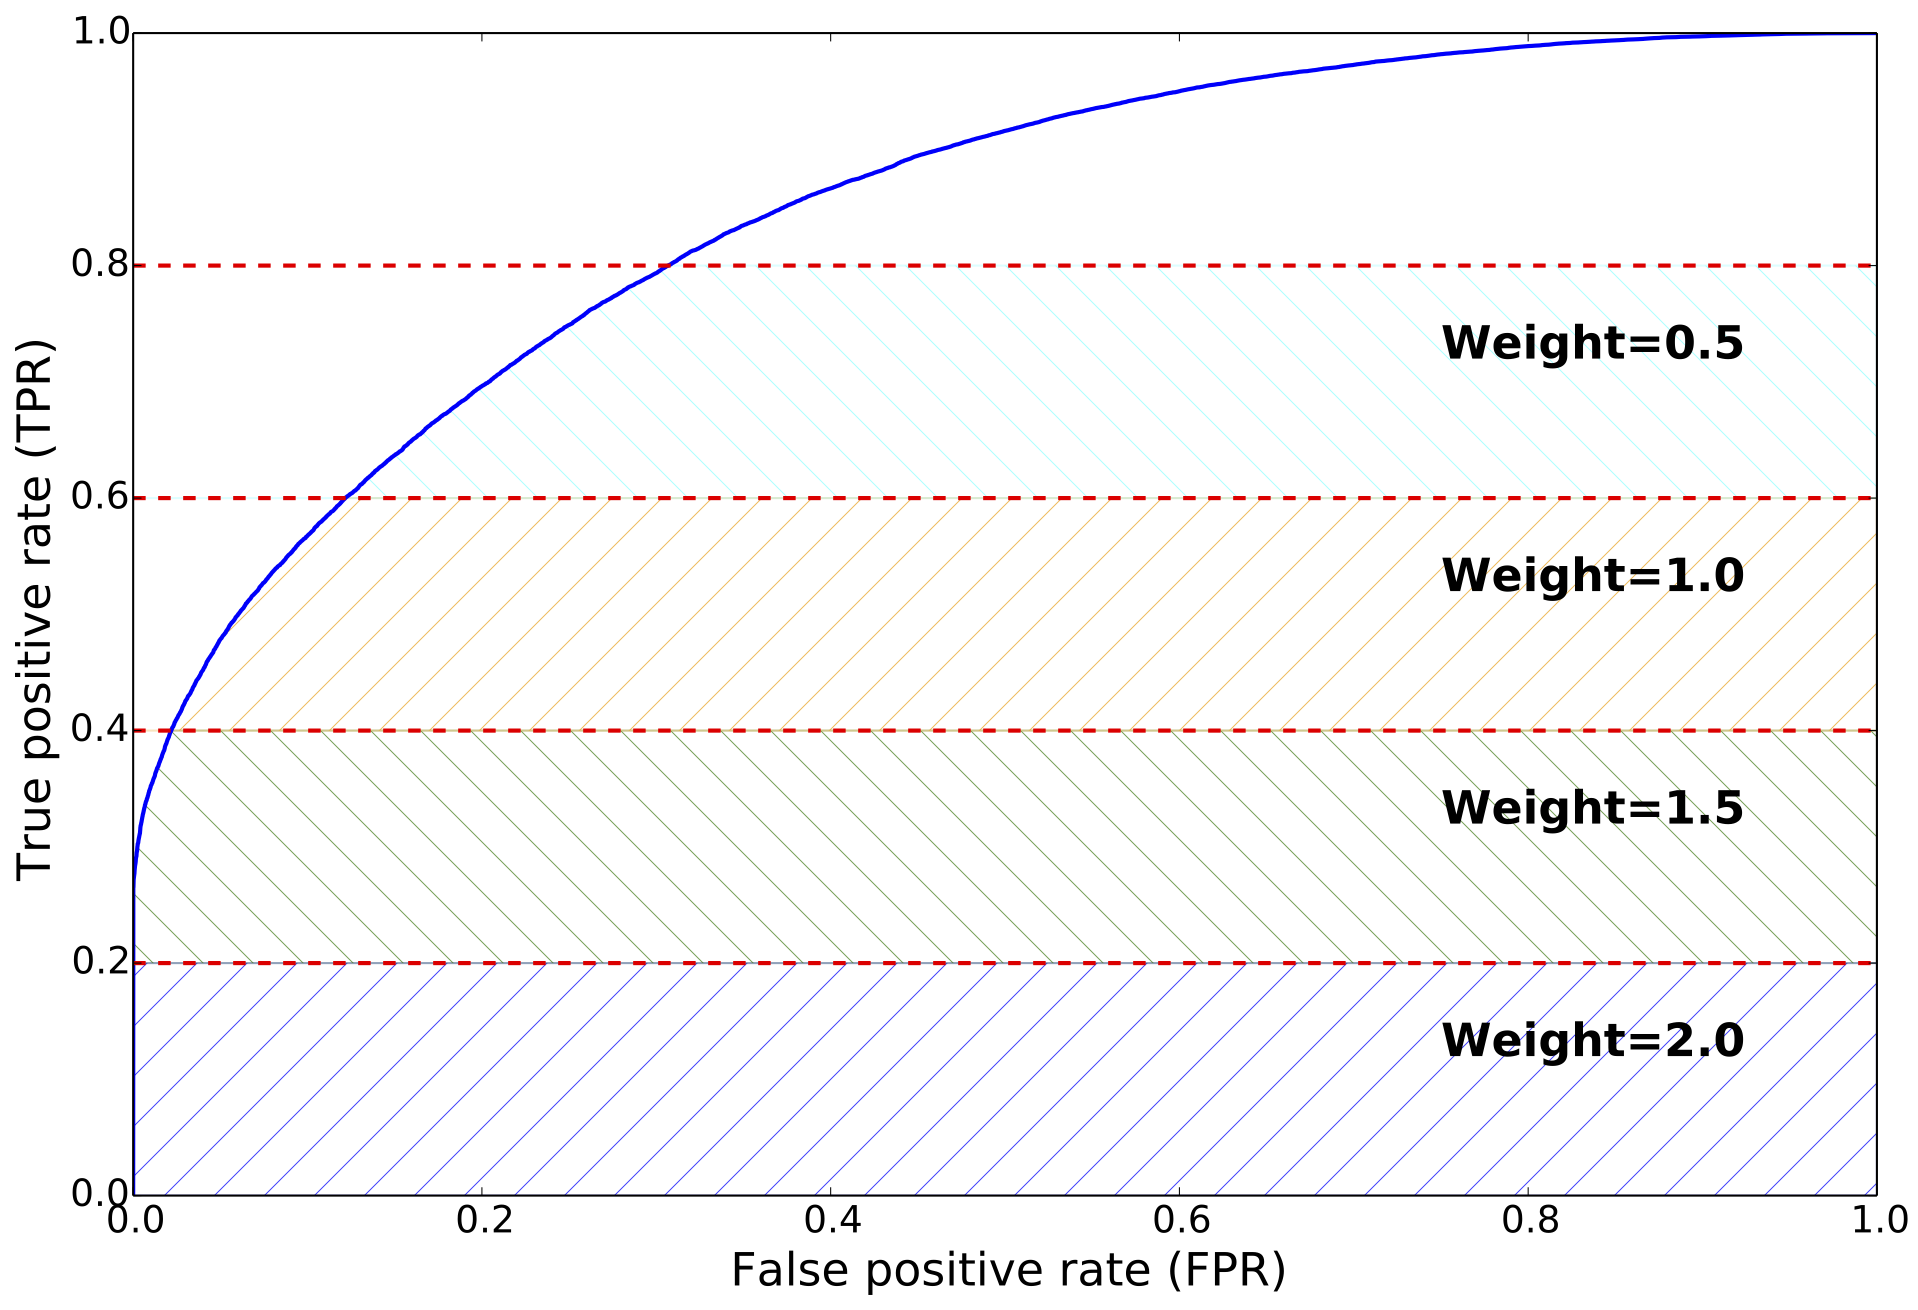
\includegraphics[scale = .3]{roc_optimistic}
\end{center} 
These weights were chosen to match the evaluation methodology used by CERN scientists.\cite{kaggleComp}.

\printbibliography

\end{document}
